\documentclass{jarticle}
\usepackage[dvipdfmx]{graphicx}

\newcommand*{\mbold}[1]{\mbox{\boldmath $#1$}}
\newcommand*{\doubleint}{\int\!\!\!\int}
\newcommand*{\trippleint}{\int\!\!\!\int\!\!\!\int}

\begin{document}

\section{}
\subsection{}
\subsection{}
Conservertive force : 
\begin{equation}\label{eq:conv_force}
	F_i = -\frac{\partial V}{\partial x_i}, ~~~~ V : scalar
\end{equation}

\subsubsection*{(a) Pysics of the sun and the earth}

Modeling :
\begin{itemize}
\item Mass of the sun $M$ is much larger than mass of the earth $m$, so,  we consider the sun is fixed to the origin of the inertial system. 
\item Diameter of the sun(1400,000km) and that of the earth(6400km) is much smaller than the distance between the sun and the earth(150000000km), so, we consider them as mass points.
\end{itemize}

Universal gravitaion force : 
\begin{equation}
	F_i = -G\frac{mM}{R^2}\frac{x_i}{R}
\end{equation}

Using eq(\ref{eq:conv_force}), 
\begin{equation}\label{eq:diff_eq}
	\frac{\partial V}{\partial x_i} = G\frac{mM}{R^2}\frac{x_i}{R} .
\end{equation}

$V$ is a function of $\{x_i\}_{i=1}^3$, then,
\[
	dV = \sum_{i=1}^3 \frac{\partial V}{\partial x_i} dx_i .
\]

Using eq(\ref{eq:diff_eq}), 
\[
	dV = GmM \sum_{i=1}^3 \frac{x_i}{R^3} dx_i = GmM \frac{\mbold{R}}{R^3}\cdot d\mbold{R}
\]

$d\mbold{R}$ is composed by the component parallel with $\mbold{R}$ and the component perpendicular with $\mbold{R}$, 
\[
	d\mbold{R} \equiv d\mbold{R}_\perp +d \mbold{R}_\parallel
\]

$\mbold{R} \cdot d\mbold{R}_\perp = 0$, then, 
\[
	dV = GmM\frac{\mbold{R}}{R^3} \cdot d\mbold{R}_\parallel = GmM\frac{1}{R^2}dR_\parallel
\]

$dR_\parallel$ is the small change of $R$, so, it can be written as $dR$. 

\[
	dV = GmM\frac{dR}{R^2}
\]

Thus, 

\[
	V = -GmM\frac{1}{R}
\]

\subsubsection*{(b) Physics of the earth and the satellite}

Modeling : 
\begin{itemize}
\item Mass of the earth $M$ is much larger than mass of the satellite $m$, so,  we consider the earth is fixed to the origin of the inertial system. 
\item The height of the satellite orbit(over 100km) is much larger than the size of satellite, so we consider the satellite as a mass point.
\item The earth is the aggregation of many($N$) small mass($m_i$). Any small mass is fixed to each position by all the other small mass.
\end{itemize}

We can choose the size of small mass so that (the size of satellite) $\ll$ (the distance between the satellite and the small mass).
Then, the situation is same as (a). The universal gravitation acting on the satellite is, 

\[
	\mbold{F} = -\sum_{i=1}^N \frac{G m m_i}{R_i^2}\frac{\mbold{R_i}}{R_i}
\]

By the same calcuration as (a), 
\[
	V = -\sum_{i=1}^N \frac{G m m_i}{R_i}
\]

\subsection{}
The density of the earth : 
\begin{equation}
	V(x,y,z) = -Gm \trippleint \frac{dx^\prime dy^\prime dz^\prime \rho(x^\prime, y^\prime, z^\prime)}{\sqrt{(x - x^\prime)^2 + (y - y^\prime)^2 + (z - z^\prime)^2}}
\end{equation}

\subsubsection*{(a) Perfect sphere, constant density}
$\rho = const$, then
\begin{equation}\label{eq:const_dens_potential}
	V(x,y,z) = -Gm\rho \trippleint \frac{dx^\prime dy^\prime dz^\prime}{\sqrt{(x - x^\prime)^2 + (y - y^\prime)^2 + (z - z^\prime)^2}}
\end{equation}

Consider polar system : 
\begin{figure}[htbp]
	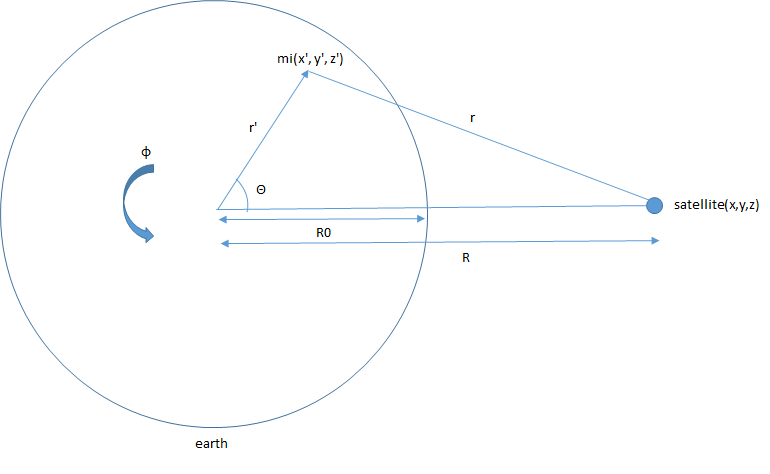
\includegraphics[width=10cm]{earth_satellite.png}
\end{figure}

On the polar system$(r^\prime, \theta, \phi)$ whose origin is the centre of the earth, the distance between the satellite and the small mass $m_i$ is, 
\begin{equation}
	r = \sqrt{r^{\prime 2} + R^2 - 2 r^\prime R \cos\theta}
\end{equation}

Jacobian is $r^{\prime 2}\sin\theta$, then
\begin{equation}
	dx^\prime dy^\prime dz^\prime = r^{\prime 2}\sin\theta drd\theta d\phi
\end{equation}

In the perfect sphere, $0 \leq r^\prime \leq R_0$, $0 \leq \theta \leq \pi$, and $0 \leq \phi \leq 2\pi$, then,  eq(\ref{eq:const_dens_potential}) can be calcurated, 
\begin{eqnarray}\label{eq:calcurated_potential}
	&&-Gm\rho \trippleint \frac{dx^\prime dy^\prime dz^\prime}{\sqrt{(x - x^\prime)^2 + (y - y^\prime)^2 + (z - z^\prime)^2}} \nonumber \\	 
	&&= -Gm\rho \int_0^{2\pi} d\phi \int_0^{R_0} dr^\prime \int_0^\pi d\theta \frac{r^{\prime 2}\sin\theta}{\sqrt{r^{\prime 2} + R^2 - 2 r^\prime R \cos\theta}} \nonumber \\	
	&&= -2\pi Gm\rho \int_0^{R_0} dr^\prime \int_{-1}^{1} \frac{-r^{\prime 2} d(\cos\theta)}{\sqrt{r^{\prime 2} + R^2 - 2 r^\prime R \cos\theta}} \nonumber\\
	&&= -2\pi Gm\rho \int_0^{R_0} dr^\prime \left[ \frac{-2r^{\prime 2} \sqrt{r^{\prime 2} + R^2 - 2 r^\prime R \cos\theta}}{-2r^\prime R} \right]_{\cos\theta = -1}^{\cos\theta = 1} \nonumber \\
	&&= \frac{2\pi Gm\rho}{R} \int_0^{R_0} dr^\prime r^\prime (|r^\prime - R| - (r^\prime + R)) 
\end{eqnarray}

The satellite is outside of the earth, then $R > R_0 \Rightarrow r^\prime < R$, eq(\ref{eq:calcurated_potential}) becomes,
\begin{equation}
	-\frac{2\pi Gm\rho}{R} \int_0^{R_0} dr^\prime 2r^{\prime 2} = -\frac{Gm}{R}\frac{4\pi R_0^3}{3}\rho = -\frac{GmM}{R}
\end{equation}

Considering the case $R < R_0$, we can calcurate the potential inside the earth. 
Eq(\ref{eq:calcurated_potential}) becomes,
\begin{eqnarray}
	V &=& \frac{2\pi Gm\rho}{R} \left[ \int_0^R dr^\prime r^\prime (-2r^\prime) + \int_R^{R_0} dr^\prime r^\prime (-2R) \right] \nonumber \\
	&=& \frac{2\pi \rho mG}{3}R^2 - 2\pi G m\rho R_0^2
\end{eqnarray}

The force is,
\begin{equation}
	\mbold{F} = -\nabla V = -\frac{2\pi \rho m G}{3}\nabla (R^2)
\end{equation} 

Using, 
\[
	(\nabla (R^2))_i = \frac{\partial}{\partial x_i}\sum_{j=1}^3 x_j^2 = 2x_i
\]

\begin{equation}
	\mbold{F} = -\frac{4\pi \rho m G}{3}\mbold{R}
\end{equation}

$\mbold{F}$ is a harmonic oscillator force. Potential has a form as $aR^2 +b$. Harmonic oscillator potential.

Simulated result is following.
\begin{figure}[htbp]
	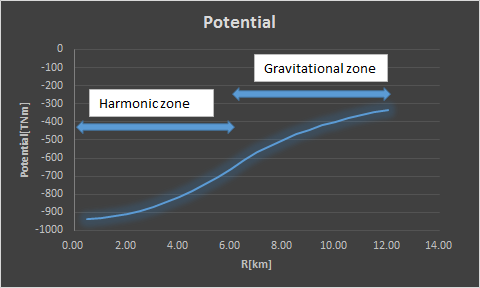
\includegraphics[width=10cm]{potential_plot.png}
\end{figure}
\begin{figure}[htbp]
	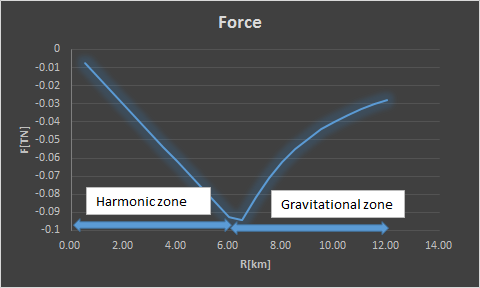
\includegraphics[width=10cm]{force_plot.png}
\end{figure}

\subsubsection*{(b) Effect of small distortion from sphere} 

\subsection{}

\subsection{}\label{subsec:1.5}
Harmonic oscillator potential :
\begin{equation}
	V(x) = \frac{1}{2}Kx^2
\end{equation}

Eq(1.42) : 
\begin{equation}\label{eq:1.42}
	t-t_0 = \pm \int_{x_0}^x \frac{1}{\sqrt{(2/m)(E-V(x))}}dx
\end{equation}

Mathmatical technique : 

\begin{eqnarray}
	\frac{d}{dx}(\sin{(\arcsin{x})}) = \frac{d}{dx}x = 1 \nonumber \\
	\cos{(\arcsin{x})}\frac{d}{dx}(\arcsin{x}) = \sqrt{1-\sin^2{(\arcsin{x})}}\frac{d}{dx}(\arcsin{x}) \nonumber \\
	= \sqrt{1 - x^2}\frac{d}{dx}(\arcsin{x}) \nonumber \\
	\Rightarrow \frac{d}{dx}(\arcsin{x}) = \frac{1}{\sqrt{1-x^2}}
\end{eqnarray}

Rightside of eq(\ref{eq:1.42}) becomes,

\begin{eqnarray}
	\int_{x_0}^x \frac{1}{\sqrt{(2E/m)}}\frac{1}{\sqrt{1 - (K/2E)x^2}}dx \nonumber \\
	= \frac{1}{\sqrt{2E/m}} \frac{1}{\sqrt{K/2E}} \int_{x_0\sqrt{K/2E}}^{x\sqrt{K/2E}}\frac{1}{\sqrt{1-x^2}}dx \nonumber \\
	= \frac{1}{\sqrt{K/m}} \left[\arcsin{(x\sqrt{K/2E})} - \arcsin{(x_0\sqrt{K/2E})}\right] \nonumber
\end{eqnarray}

Select $t_0 = 0$, 
\begin{eqnarray}
	\omega t = \arcsin{(x\sqrt{K/2E})} - \arcsin{(x_0\sqrt{K/2E})} \nonumber \\
	\Rightarrow x = \sqrt{\frac{2E}{K}} \sin{\left(\omega t + \arcsin{(x_0\sqrt{K/2E})}\right)}
\end{eqnarray}

To set to same form as eq(1.44), 
\begin{eqnarray}
	x = \sqrt{\frac{2E}{K}}\sin\left(\omega t + \frac{\pi}{2} + \arcsin(x_0\sqrt{K/2E}) - \frac{\pi}{2}\right) \nonumber \\
	= \sqrt{\frac{2E}{K}}\sin\left(\omega t + \frac{\pi}{2} + \arccos(x_0\sqrt{K/2E})\right) \nonumber \\
	= \sqrt{\frac{2E}{K}}\cos(\omega t + \gamma), ~~~~~~~~ \cos\gamma = x_0\sqrt{K/2E} \nonumber \\
	p = m\dot{x} = -m\omega \sqrt{\frac{2E}{K}}\sin(\omega t + \gamma)
\end{eqnarray}

All phase space streamline of this system create concentric ellipses. For example, consider a group of initial values, which creates a ellipse sector angle $\theta$. This group creates a space $\Gamma_0$ in phase space. 

Area of $\Gamma_0$ is $2m\omega E\theta /K$. After $t$[sec], any point in the group rotates $\omega t$, along each streamline. Thus, $\theta$ doesn't change($\Gamma_t = \Gamma_0$) : Liuville's theorem.

\subsection{}
Electric potential : 
\[
	V(x) = -eV\left(1 - \frac{|x|}{a}\right)
\]

For this potential, $x=0$ is a singular point. 

Force : 
\begin{equation}\label{eq:equation_of_motion}
	\dot{p}^2 = F(x) = -eV\frac{{\rm sign}(x)}{a}, ~~~~ x\neq 0
\end{equation}

Conservation of energy : 
\begin{equation}\label{eq:conserv_energy}
	\frac{1}{2m}p^2 -eV\left(1-\frac{|x|}{a}\right) = E
\end{equation} 

At initial, $p(0) = 0$, $x = b$, then, 
\[
	E = -eV\left(1-\frac{b}{a}\right)
\]

Eq(\ref{eq:conserv_energy}) becomes.
\begin{eqnarray}\label{eq:phase_space_equation}
	\frac{1}{2m}p^2 + eV\frac{|x|}{a} = eV\frac{b}{a} \nonumber \\
	\Leftrightarrow x = \pm \left(b - \frac{1}{2meV}p^2 \right)
\end{eqnarray}

\begin{figure}[htbp]
	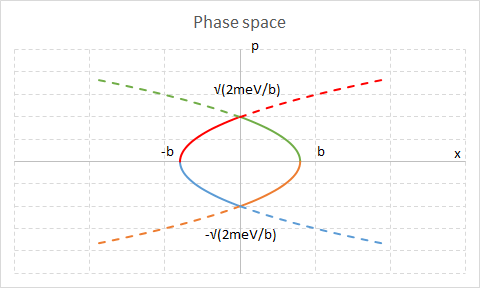
\includegraphics[width=10cm]{phase_space_plot.png}
\end{figure}

Eq(\ref{eq:phase_space_equation}) has two degrees of freedom of the sign($\pm$ and $p^2$). So, from the view point of mathmatics, 4 solutions are allowed. 
We can choose one soluton by the initial condition : 
\begin{equation}\label{eq:initial_condition}
	x(0) = b, p(0) = 0, t=0
\end{equation}
and by the equation of motion : eq(\ref{eq:equation_of_motion}).

At $t=0$ the initial condition eq(\ref{eq:initial_condition}) shows, the streamline must be started along the orange solid line or green solid line. Also, eq(\ref{eq:equation_of_motion}) shows, $p$ must be reduced. Thus, the orange solid line is selected for the stream line, and the direction is right to left. This is effective until $x=+0$. 
At $x=-0$, allowed line is the blue solid line and the orange dot line, because streamline must be continuous. Eq(\ref{eq:equation_of_motion}) shows $p$ must be increased. So, the blue solid line is selected, and the direction is still right to left. After $x = -b$, the red solid line is selected because the streamline must be continuous. 
By same logic, the green solid line is selected. 
Thus, the streamline is the solid line loop, and the direction is right rotation.

\subsection{}
2-dimentional harmonic oscillator : 
\begin{eqnarray}
	\mbold{F} = -\left(\begin{array}{c} ax \\ by \end{array} \right) \nonumber
\end{eqnarray}

Equation of motion : 
\begin{eqnarray}
	m\left( \begin{array}{c} \ddot{x} \\ \ddot{y} \end{array} \right) =  -\left(\begin{array}{c} ax \\ by \end{array} \right) \nonumber
\end{eqnarray}

Analogy with sec(\ref{subsec:1.5}), 
\begin{eqnarray}
	x = \sqrt{\frac{2E_x}{a}}\cos(\omega_x t + \gamma_x), ~~~~ \cos\gamma_x = x_0\sqrt{a/2E_x},~~~ E_x = \frac{1}{2m}p_{x0}^2 + \frac{1}{2}ax_0^2 \nonumber \\
	y = \sqrt{\frac{2E_y}{b}}\cos(\omega_y t + \gamma_y), ~~~~ \cos\gamma_y = y_0\sqrt{b/2E_y},~~~ E_y = \frac{1}{2m}p_{y0}^2 + \frac{1}{2}ay_0^2 \nonumber 
\end{eqnarray}
where, $\omega_x = \sqrt{a/m}$, $\omega_y = \sqrt{b/m}$.

\subsubsection*{(i) $a = b$}
In this case, $\omega_x = \omega_y = \omega$, so, the differences between $x$ and $y$ are only amplitude and phase.
$A \equiv \sqrt{\frac{E_x}{a}}$, $B \equiv \sqrt{\frac{E_y}{b}}$, using additional theorem, 
\begin{equation}
	\frac{y}{B} = \frac{x}{A}\cos(\gamma_y-\gamma_x) - \sin(\gamma_y - \gamma_x)\sqrt{1-\frac{x^2}{A^2}}
\end{equation}
Delete square root, 
\begin{eqnarray}
	\frac{y^2}{B^2} +\frac{x^2}{A^2}\cos^2(\gamma_y - \gamma_x) - 2\frac{xy}{AB}\cos(\gamma_y - \gamma_x) = \sin^2(\gamma_y - \gamma_x)\left(1-\frac{x^2}{A^2}\right) \nonumber \\
	\frac{x^2}{A^2} + \frac{y^2}{B^2} -2\frac{xy}{AB}\cos(\gamma_y - \gamma_x) = \sin^2(\gamma_y - \gamma_x) \nonumber
\end{eqnarray}

If $\gamma_y = \gamma_x$, it means $x_0 = y_0$ and $E_x = E_y$, 
\[
	\frac{x}{A} - \frac{y}{B} = 0
\]
Thus, this is a straight line.
If $\gamma_y \neq \gamma_x$, 
\[
	\frac{1}{A^2}\frac{1}{B^2} - \left( \frac{\cos(\gamma_y - \gamma_x)}{AB} \right)^2 >0
\]
then, this is a ellipse with slope.

\begin{figure}[htbp]
	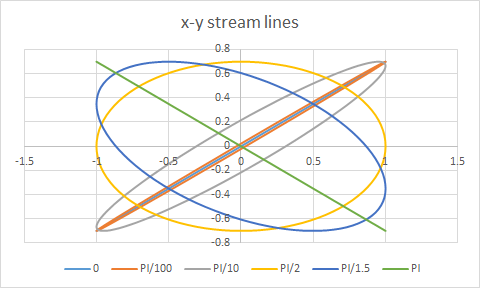
\includegraphics[width=10cm]{two_dim_harmonic_streamline.png}
\end{figure}

\subsubsection*{(ii) $a = 4b$}
$\omega_x = 2\omega_y$. In this case, streamline draws a bit complicated line. 
\begin{figure}[htbp]
	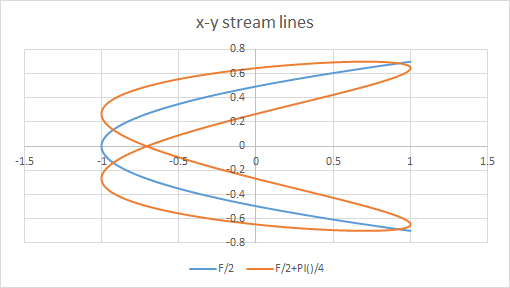
\includegraphics[width=10cm]{two_dim_harmonic_streamline_div4.png}
\end{figure}
If $\gamma_y=\gamma_x$, the line is parabola, because, $\cos2\omega t = 2\cos^2\omega t - 1$. 
The stream line is periodic. The period of $x$ is $T_x = 2\pi/\omega_x$, the otherhand, the period of $y$ is $T_y = 2\pi/\omega_y = T_x/2$. So, $2T_x$ is the period of whole system. 

\subsubsection*{(iii) General case}
If $\omega_x / \omega_y$ is a fraction($\sqrt{a/b}$ is a fraction), with analgy with (ii), the streamline is periodic and the period is LCM of $\omega_x$ and $\omega_y$. 
But if $\omega_x / \omega_y$ is a irrational number, the streamline is never periodic. Thus, the streamline never passes same point. 

\begin{figure}[htbp]
	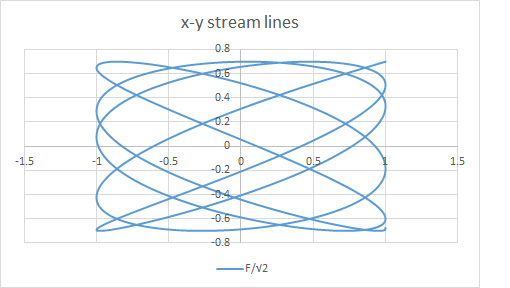
\includegraphics[width=10cm]{two_dim_harmonic_streamline_divsqrt2.png}
\end{figure}
\end{document}